\section{Objektorientierte Modelle und Operationen}

\subsection{Konzepte objektorientierter Programmiersprachen}
\begin{itemize}
	\item starker Einfluss der OO DB-Modelle durch OO Systeme
	\item \textbf{Entwurfsphasen}
	\begin{enumerate}
		\item Identifiziere Objekte der Anwendung
		\item Beschreibe Objekte der Anwendung
		\item Identifiziere Beziehungen und Gemeinsamkeiten zw Objekten
		\item Fasse Objekte mit gemeinsamen Eigenschaften zu Klassen zsm
		\item Identifiziere Beziehungen zw Klassen
		\item Bilde Klassenhierarchien
		\item Implementiere die Funktionen einzelner Klassen
		\item Entwickle Programme aus Objektbeschreibungen
	\end{enumerate}
	Phase 2 bis 4 möglichst mit \textit{abstrakten Datentypen}\\
	\textit{Typen:} generischer Typ T, beschreibt Menge von Objekten, ein Objekt heißt Instanz\\
	\textit{Funktionen:} Operationen durch Signatur beschrieben (Typen des Def.- und Bildbereichs); formal seiteneffekt-frei (verändern nie ein Argument)\\
	\textit{Vorbedingungen:} insbesonderefür partielle Fkt (bsp: Kelleroperation top(), nur anwendbar, wenn Keller nicht leer)\\
	\textit{Axiome:} Semantikbeschreibung von Fkt, Festlegung des Verhaltens 
\end{itemize}

\subsubsection{Prinzipien des OO Entwurfs}
\begin{itemize}
	\item Klassen sind ADT-Implementierungen (meist ohne Axiome, Vorbedingungen)
	\item Beziehungen zw Klassen:\\
	Klasse - Komponentenklasse: wird zur Implementierung einer anderen Klasse benutzt\\
	Komponentenobjekt: im  Zustand eines anderen Objekts\\
	Klasse- Unterklasse: steuert die Vererbung von Attributen und Methoden
	\begin{figure}[!h]
		\centering
		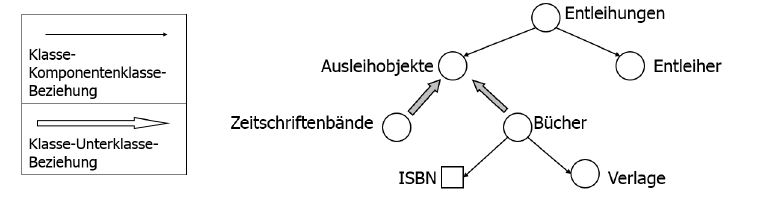
\includegraphics[scale=0.5]{img/adt_inherit_components.png}
	\end{figure}
\end{itemize}

\textbf{Attribute und Methoden}\\
Komponenten eines Objekttyps
\begin{itemize}
	\item Attribute: Eigenschaften von Objekten
	\item Methoden: auf Objekten durchführbare Funktionen
\end{itemize}

\textbf{Einkapselung}
\begin{itemize}
 	\item Schnittstelle (public): Methodensignatur (Eingabe, Ausgabe) -> Protokoll einer Botschaft
	\item Implementierung (private): Attribute und Methodenimplementierung
	\item Methodenaufruf: Senden einer Botschaft mit \textit{Objekt.Methode} -> Objekt ist Empfänger der Botschaft
	\item Klasse: Menge von Objekten mit gleichen Attributen und Methoden\\
	Programmiersprachen: Klasse ist Implementierung eines ADT\\
	DB: Klasse ist Objektfabrik (und -lager)
\end{itemize}

\textbf{Konstruktor und Destruktor}\\
Zum Erzeugen (Konstruktor; zusätzlich Initialisierung des Objekts) und Löschen eines Objekts (Destruktor)\\
\\
\textbf{Zuweisung:}\\
Unterscheidung zw Wert und Referenzsemantik
\begin{figure}[!h]
	\centering
	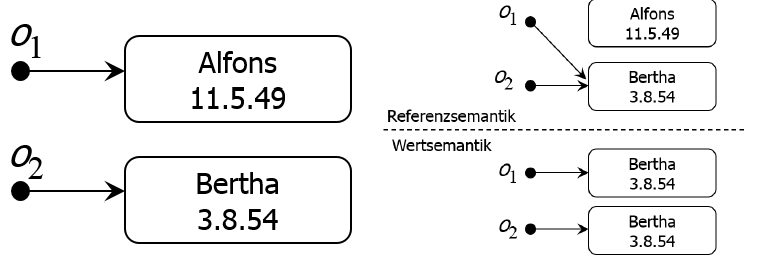
\includegraphics[scale=0.5]{img/value_ref_semantics.png}
	\caption{Unterscheidung Zuweisung Wert- und Referenzsemantik}
\end{figure}

\textbf{Kopieren}
\begin{itemize}
	\item Flaches kopieren: lediglich Verweis auf die Referenz des zu kopierenden Objektes; Originalobjekt und Kopie teilen sich Attribute
	\item Deep Copy: zusätzliche Kopie der Attribute -> Original und Kopie teilen sie nicht
\end{itemize}

\textbf{Identität}
\begin{itemize}
	\item Objekte identisch: gleiche Referenz
	\item Objekte oberflächlich gleich: gleichen Zustände
	\item Objekte in der Tiefe gleich: rekursiv gleiche Zustände
\end{itemize}

\textbf{Typisierung}
\begin{itemize}
	\item statisch: Typ jedes Ausdrucks zur Übersetzungszeit bekannt
	\item streng: keine Typfehler zur Laufzeit (Bsp: C++, Eiffel)
\end{itemize}

\textbf{Vererbung}
\begin{itemize}
	\item Weitergabe von Attributen und Methoden von Ober- zu Unterklasse
	\begin{table}[!h]
		\begin{tabular}{|l|p{30em}|}
			\hline
			Begriff	& Haupteigenschaft\\
			\hline
			\hline
			Spezialisierung	& Integritätsbedingungen: Objektmenge der Unterklasse ist Teilmenge der Objektemenge in der Oberklasse\\
			\hline
			IST-Hierarchie	& wie Spezialisierung\\
			\hline
			Typhierarchie	& Gleiches Verhalten: jedes Objekt des Untertyps verhält sich wie eines des Obertyps\\
							& Alle Attribute und Methoden des Obertyps sind auf Objekte des Untertyps anwendbar\\
							& Substitution: jedes Objekt des Untertyps kann für bel. Objekt des Obertyps eingesetzt werden\\
			\hline
			Klassenhierarchie	& Vererbung der Implementierung: Unterklasse wird mit Hilfe der Datenstrukturen für Attribute und Implementierung von Methoden aus der Oberklasse impl\\
			\hline
		\end{tabular}
	\end{table}
	
	\begin{figure}[!h]
		\centering
		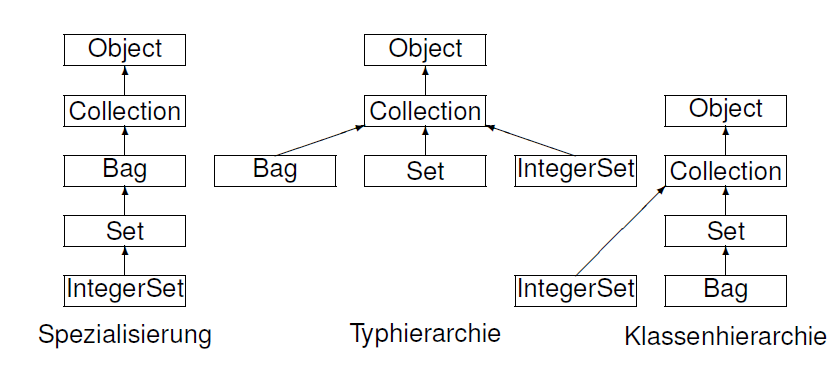
\includegraphics[scale=0.6]{img/oopl_inheritance.png}
		\caption{Vererbung Unterschiede am Bsp}
	\end{figure}
	
	\item Mehrfachvererbung: Klasse darf mehrere Oberklassen haben\\
	Probleme: Konflikte bei gleicher Methodensignatur -> Vermeidung oder Auflösung bspw. durch REDEFINE einer Methode
\end{itemize}

\textbf{Overriding}
\begin{itemize}
	\item Oberklasse: Methode M, Implementierung MI1
	\item Normalfall der Vererbung: Unterklasse erbt Methode M, Implementierung MI1
	\item \textbf{Overriding:} Unterklasse erbt Methode M, ersetzt Implementierung durch MI2 => erfordert dynamisches Binden
	\item Varianten des Overriding:
	\begin{itemize}
		\item \textit{Ersetzung:} völlige Ersetzung von MI1 durch MI2\\
		Bsp: Eiffel REDEFINE
		
		\item \textit{Verfeinerung:} MI1 wird von MI2 aufgerufen 
	\end{itemize}
\end{itemize}

\textbf{Polymorphismus und dynamisches Binden}
\begin{itemize}
	\item Methode polymorph: kann auf Objekte unterschiedlicher Klasse angewandt werden => Wiederverwendbarkeit\\
	Bsp: Addition -> unterschiedliche Impl je nach Datentyp
	
	\item dazu notwendig: dynamisches Binden:\\
	Auflösung eines Methodenaufrufs (dessen Impl) zur Laufzeit anhand des Objekttyps
\end{itemize}

\textbf{Vergleich OOPL und OO DB-Modelle}
\begin{table}[!h]
	\centering
	\begin{tabular}{|p{10em}|p{15em}|p{15em}|}
		\hline
		Eigenschaft	& OOPL	& OODM \\
		\hline
		\hline
		Attribute, Methoden, Typisierung	& untypisiert oder wenig orthogonales Typkonzept; mengen oft durch generische Klassen simuliert & orthogonales Typkonzept zur Darstellung komplexer Werte\\
		\hline
		Einkapselung	& Attribute sollen privat sein	& Attribute und Datentypen wahlweise bekannt -> Unterstützung von Anfragen und Zugriffspfaden\\
		\hline
		Klassen & Implementierung eines ADT	& Objektfabrik und -lager, das automatisch verwaltet wird\\
		\hline
		Konstruktoren \& Destruktoren	& Objekt wird erzeugt und ''klebt'' an seiner Klasse & Objekt wird erzeugt, kann aber zu mehreren Klassen gehören und diese auch wechseln\\
		\hline
		Vererbung	& Klassenhierarchie = Vererbung der Impl	& Klassenhierarchie = Spezialisierung\\
																&& Typhierarchie = Erweiterung der anwendbaren Attribute, Methoden\\
		\hline
	\end{tabular}
\end{table}
Zusätzlich in OODMS notwendig: \\
generische Operationen: sicher, optimierbar, deskriptiv; Definieren Relationen, dynamische Klassen; in OOPLs simuliert: Methoden auf Mengen(=generische Klassen) \\
Transaktionskonzept, Flexible Speicherungsstruktur

\subsection{Einschub}

\subsubsection{''Reines'' OO programmieren mit Smalltalk}
Eigl nur konkrete Umsetzung des vorherigem anhand von Smalltalk. Denke nicht, das dies prüfungsrelevant ist.
\begin{itemize}
	\item Alle  Elemente der Sprache sind Objekte => Kommunikation dazwischen nur Botschaften
	\item ausschließlich dynamisches Binden
	\item \textbf{Klassen}
	\begin{itemize}
		\item Klasse ist Instanz ihrer Metaklasse
		\item besteht aus: Instanzvariablen (Zustand jedes Objekts)\\
		Klassenvariablen (Zustand der Klasse als Objekt)\\
		Instanzmethoden (kann jedes Objekt der Klasse ausführen)\\
		Klassenmethoden (kann die Klasse ausführen)
		\item Klassenhierarchie: Baum mit Wurzel \textit{Object}
	\end{itemize}
	
	\item Smalltalk kennt nicht:\\
	Typisierung\\
	Mehrfachvererbung\\
	Gesteuerte Vererbung\\
	Öffentliche Attribute\\
	Statisches Binden
\end{itemize}

\subsubsection{Ist C++ streng typisiert?}
streng typisiert = keine Typfehler zur Laufzeit\\
Problem (?) bei
\begin{itemize}
	\item statisch erzeugten Objekten
	\item Zuweisung mit Wertsemantik
	\item Vererbung und Overriding
\end{itemize}
Fazit: Fehler nicht nachweisbar in neuen Versionen 

\subsection{Ein objektorientiertes Datenbankmodell: Überblick}
\begin{framed}
	\textbf{Definiton 1}
\begin{description}
	\item Ein OODBS ist ein System, das
	\begin{itemize}
		\item auf einem OODM basiert
		\item erweiterbar ist (zumin. konzeptuell)
		\item weitere DB-Eigenschaften besitzt,
		\begin{itemize}
			\item Persistenz
			\item Speicherungsstrukturen, Zugriffspfade
			\item Transaktionen, Concurrency Control
			\item Recovery
		\end{itemize}
		\item neben generischen Operationen (etwa Anfragesprache) auch eine komplette Programmier-Umgebung beeinhaltet.
	\end{itemize}
\end{description} 
\end{framed}

\textit{Beispiel in $O_2$ - Methoden, Vererbung}
\begin{lstlisting}
CLASS Studenten INHERITS Personen
	TYPE TUPLE
		(Matrikelnummer: INTEGER,
		.....)
	METHOD Zur_Verfuegung: REAL END
	
METHOD BODY Zur_Verfuegung: REAL IN CLASS Studenten
	{ RETURN (SELF.Vater.Zur_Verfuegung +
	 SELF.Mutter.Zur_Verfuegung) * 0.1;\}
\end{lstlisting}

\subsection{Strukturteil eines OODM}
\begin{framed}
	\textbf{Definition 2 - Strukturteil OODM}
	\begin{description}
		\item Der Strukturteil eines objektorientierten Datenbankmodells besteht aus
		\begin{itemize}
			\item Typen und Typkonstruktoren
			\item Objektidentität
			\item Klassen und Typen
			\item Beziehungen zwischen Klassen
			\item Klassen- und Typhierarchie
			\begin{itemize}
				\item Strukturvererbung
				\item Mehrfachvererbung
				\item Konfliktauflösung bei Mehrfachvererbung
			\end{itemize}
			\item Integritätsbedingungen
		\end{itemize}
	\end{description}
\end{framed}

\subsubsection{Typkonstruktoren}
\begin{framed}
	\textbf{Definition 6 - Typen und Typkonstruktoren}
	\begin{description}
		\item An Typen stehen im OODM zur Verfügung:
		\begin{itemize}
			\item Standard-Datentypen \textit{integer, string,...,} die für das OODM elementar und vordefiniert sind
			\item ADT \textit{DATE, TIME, ...,} die mit ilfe von Typen und Typkonstruktoren gebildet wurden entweder vordefiniert oder benutzerdefiniert sind
		\end{itemize}
		
		\item sowie alle Typen, die mit den obigen Typen und
		\begin{itemize}
			\item Typkonstruktoren \textit{TUPLE OF, SET OF, LIST OF, BAG OF, ARRAY OF}
		\end{itemize}
		\item definiert wurden. Die Typkonstruktoren sind dabei orthogonal anwendbar.
	\end{description}
\end{framed}

\begin{itemize}
	\item Nach Beeri: SET OF, TUPLE OF orthogonal anwendbar (komplexe Werte)
	\item Geschachtelte Relationen (NF2-Relationen): SET OF TUPLE OF (Relationenkonstruktor)
	\item Komplexe Werte und geschachtelte Relationen äquivalent vom Informationsgehalt her
	\begin{lstlisting}
		SET OF (TUPLE OF (Name: TUPLE OF(...)))
	\end{lstlisting}
	\item Relationenmodell: nur SET OF TUPLE OF <Standard-Datentyp>
	\item OOPL: nicht typisiert; nicht orthogonal; einige Konstruktoren nur simulierbar
	\item rekursive Typdefinitionen (Personen: SET OF TUPLE OF (...Freunde: Personen)) nicht erlaubt, besser durch Objektidentität auflösen (sonst endlos)
	\item Simulation der Typkonstruktoren in C++
	\begin{itemize}
		\item statt Typkonstruktor: generische Klasse
		\item Nachteile: nicht fest verdrahtet im System; kann redefiniert werden\\
		Duplikateliminierung nicht automatisch mgl; Semantik einer Menge nicht bekannt
	\end{itemize}
	\item \textbf{Operationen}
	\begin{itemize}
		\item Tupelkonstruktor: Komponentenzugriff; Test auf (Un-)Gleichheit 
		\item Mengenkonstruktor: Zugriff auf ein Element: Iteratoren\\
		Test auf ein Element\\
		Vergleich von Mengen mit $=, \neq, \subset \subseteq,$ und deren Negationen\\
		Mengenoperationen Vereinigung, Durchschnitt und Differenz
		\item Listenkonstruktor: Zugriff auf erstes (first), nächstes (next), letztes (last) Element\\
		Teilliste erstellen ohne erstes Element (tail)\\
		Iterator zum Durchlaufen der Liste in vorgegebener Reihenfolge\\
		Konkatenation von Listen
	\end{itemize}
	
	\item \textbf{Grenzen}
	\begin{itemize}
		\item Redundanzen bei nichthierarchischen Strukturen
		\item geschachtelte Relationen können redundanzfrei nur rein hierarchische Objektmengen darstellen
		\item darum Objektidentität notwendig
	\end{itemize}
\end{itemize}

\begin{figure}[!h]
	\centering
	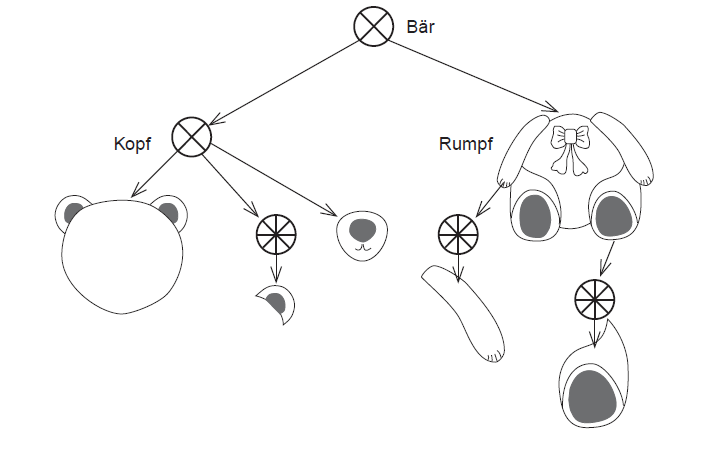
\includegraphics[scale=0.5]{img/struc_1.png}
\end{figure}

\subsubsection{Objektidentität}
\begin{framed}
	\textbf{Definition 3 - Objektidentität}
	\begin{description}
		\item Eine Objektidentität ist ein \textit{abstrakter} Wert, der für jedes Objekt der Datenbank
		\begin{itemize}
			\item bei Erzeugen dieses Objektes vom System vergeben wird,
			\item systemweit eindeutig ist,
			\item unveränderbar ist,
			\item von außen nicht sichtbar ist.
		\end{itemize}
	\end{description}
\end{framed}

\begin{itemize}
	\item daher Beziehungen zw Objekten darstellbar, etwa eine gemeinsame Komponentenobjekte
	\item bei einigen System von außen sichtbar: dann gelöschte Objektidentitäten nicht wiederverwendbar
	\item \textbf{Unterscheidung Werte - Objekte}
	\begin{table}[!h]
		\centering
		\begin{tabular}{|p{20em}|p{20em}|}
			\hline
			Objekt	& Wert\\
			\hline
			\hline
			nicht druckbar	& druckbar\\
			\hline
			anwendungsabhängige Abstraktion	& anwendungs\textit{un}abhängige Abstraktion\\
			\hline
			müssen erzeugt und definiert werden & müssen \textit{nicht} erzeugt und definiert werden\\
			\hline
			trägt selsbt keine Information & trägt Information\\
			\hline
			werden beschrieben & beschreiben etwas\\
			\hline
		\end{tabular}
	\end{table}

	Danach sind Werte Element von unstrukturierten (atomaren), konkreten Menge, den Domänen von Std-Typen etwa oder\\
	strukturierten Mengen, die mittels TUPLE OF, SET OF, LIST OF oder anderen Typkonstruktoren erzeugt werden (in denen dann neben Werten auch wieder Objekte vorkommen können)
	
	\item \textbf{Zuordnung Objekte - Zustände}
	\begin{itemize}
		\item Zustand eines Objekte $o$\\
		- komplexe Werte\\
		- andere (Komponenten-)Objekte ($o$ heißt dann zusammengesetztes Objekt)
		
		\item Darstellung von Objekten mit Zustand\\
		Objekt (kleiner Kreis), Zurodnung des Zustands (Pfeil), Zustand (Oval)\\
		geschachtelte Relationen mit spezieller Spalte für Objektidentitäten (Objektrelationen)
	\end{itemize}
	
	\item \textbf{Unterschiede, Einordnungen}
	\begin{itemize}
		\item Relationenmodell
		\begin{itemize}
			\item Objekte nur über siuchtbare Schlüssel und Fremdschlüssel zu identifizieren
			\item veränderbar
			\item nur relationenweit eindeutig
			\item vom Nutzer vergeben
		\end{itemize}
		\item OOPLs
		\begin{itemize}
			\item Objektidentität meist physischer Zeiger, der aber veränderbar ist
			\item ein Objekt kann nicht in mehreren Klassen mit der gleichen Identität auftauchen
		\end{itemize}
	\end{itemize}
	
	\item \textbf{Realisierungen}
	\begin{itemize}
		\item Abstrakte Objekte
		\begin{itemize}
			\item Elemente einer globalen Menge abstrakter Objekte
			\item Elemente verschiedener, disjunkter, abstrakter Domänen
		\end{itemize}
		
		\item Surrogat-Attribute
		\begin{itemize}
			\item beste Implementierung von abstrakten Objekten
			\item als konzeptuelle Objektidentität mit Vorsicht zu behandeln (Sichtbarkeit, Änderbarkeit, funktionale Beziehungen zu Zuständen)
		\end{itemize}
		
		\item Namen
		\begin{itemize}
			\item zur Zusatz-Identifikation einiger Objekte geeignet
			\item problematischer Test auf Identität (mehrere Namen für ein Objekt)
		\end{itemize}
		
		\item direkte oder indirekte Referenzen
		\begin{itemize}
			\item nur als Implementierungshilfsmittel geeignet
			\item indirekte Referenzen sind flexibler (Verschiebbarkeit von Objekten)
		\end{itemize}
	\end{itemize}
\end{itemize}

\begin{figure}[!h]
	\centering
	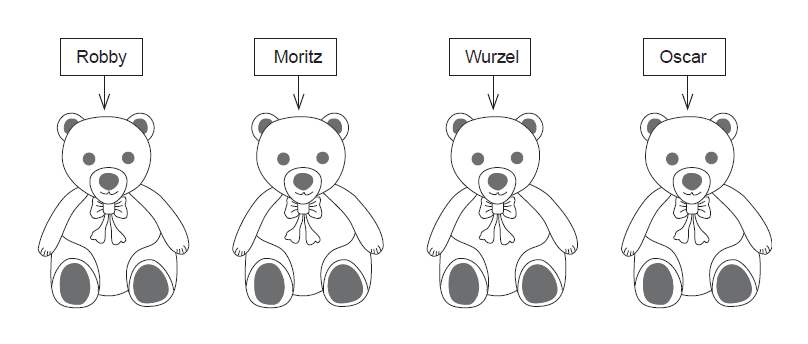
\includegraphics[scale=0.5]{img/struc_2.png}
\end{figure}

\subsubsection{Klassen und Typen}
\begin{framed}
	\textbf{Definition 4 - Klassen, Zustände, Zustandstypen}
	\begin{description}
		\item eine Klasse besteht aus
		\begin{itemize}
			\item einer abstrakten Domäne (der Wertevorrat der Objektidentitäten)
			\item einer Extension (auch: Instanz), also der aktuellen Objektmenge = Menge bislang erzeugter und noch nicht gelöschter Objekte (= Persistenz)
			\item einem zugeordneten Zustandstype (mit Typen und Typkonstruktoren)
			\item einer Zuordnung von Zuständen zu Objekten
		\end{itemize}
	\end{description}	
\end{framed}
\begin{itemize}
	\item ein Objekte kann in mehreren Klassen vorkommen (mehrere ROllen spielen: Person, Student, Angestellter,...)
	\item spielt dann mehrere Rollen durch Ober- und Unterklassen
	\begin{figure}[!h]
		\centering
		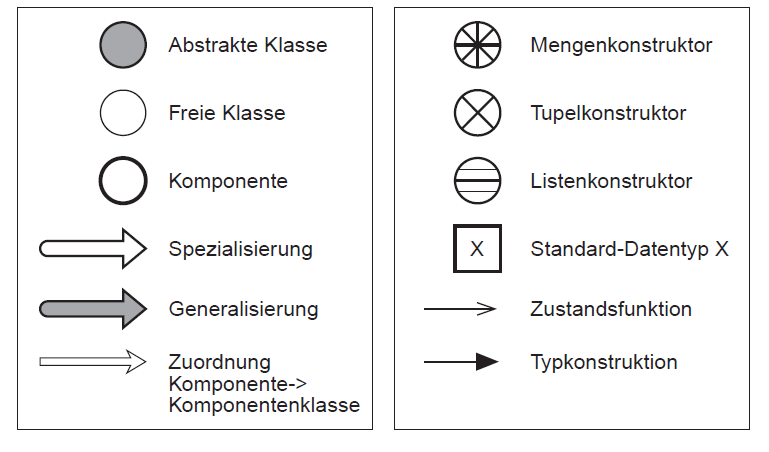
\includegraphics[scale=0.5]{img/legend_oodm.png}
		\caption{Grafische Symbole für OODM}
	\end{figure}
	
	\item \textbf{Beispiel}\\
	Der Klasse \textit{Bücher} ordnen wir die folgenden Informationen zu:
	\begin{itemize}
		\item die abstrakte Domäne $\{\alpha_1, \alpha_2, \ldots\}$, \textit{Bücher} ist abstrakte Klasse (s.u.)
		\item die Extension (aktuelle Objektmenge), zunächst leer, nach zehnmaliger Anwendung der Erzeugungsfunktion CREATE etwa $\alpha_1, \alpha_2, \ldots, \alpha_10$
		\item den Zustandstyp
		\begin{lstlisting}
		TUPLE OF (
			ISBN: STRING,
			Titel: STRING,
			Verlag: Verlage,
			Autoren: LIST OF (Autor: STRING),
			Stichworte: SET OF (Stichwort: STRING),
			Versionen: SET OF (TUPLE OF (Auflage: integer, Jahr: integer))
		)
		\end{lstlisting}
		der jedem Buch $\alpha$ ein Tupel zuordnet, das unter anderem wieder ein Objekt der Klasse \textit{Verlag} beinhaltet.
	\end{itemize}
	
	\item \textbf{Unterschiede und Einordnungen}
	\begin{itemize}
		\item Relationenmodell: Relation sammelt Werte, keine Objekte
		\item OOPLs: keine Instanz, wird meist explizit in Variable vom SET OF- Typ gesammelt\\
		Objekte nur in einer klasse\\
		kann keine unterschiedlichen Rollen spielen
	\end{itemize}
	
	\item zwei Arten von Klassen\\
	\textbf{Abstrakte Klasse:} wird eine abstrakte Domäne zugeordnet; hier gibt es Konstruktoren, hier werden Objekte in der DB erzeugt\\
	\textbf{Freie Klasse:} wird \textit{keine} abstrakte Domäne zugeordnet, erhält Domäne durch Vererbung, hier gibt es keine Konstruktoren, hier werden schon in der DB bestehende Objekte neu aufgenommen
\end{itemize}

\subsubsection{Beziehungen zwischen Klassen}
\begin{framed}
	\textbf{Definition 5 - Beziehungen}
	\begin{description}
		\item Eine Klasse kann in Beziehung zu anderen Klassen, ein Objekt in Beziehung zu anderen Objekten stehen. Hat eine Klasse $K_1$ eine Komponentenklasse $K_2$, so nennt man die Objekte in $K:1$ zusammengesetzte Objekte mit den zugehörigen Komponentenobjekten aus $K_2$. Komponentenklassen können folgende Eigenschaften haben:
		\begin{itemize}
			\item \textit{gemeinsam (shared)} oder \textit{privat}
			\begin{itemize}
				\item gemeinsam: ein Komponentenobjekt in vielen zusammengesetzten Objekten
				\item private: ein Komponentenobjekt in maximal einem zusammengesetzten Objekt (ACHTUNG: nicht OOPL Einkapselung privat)
				\item Bsp: Verlage gemeinsam in Bücher, Motor privat in Autos
			\end{itemize}
			
			\item \textit{abhängig} oder \textit{unabhängig}
			\begin{itemize}
				\item abhängig: Komponentenobjekt wird gelöscht, wenn (letztes) zugehöriges zusammengesetztes Objekt gelöscht wird
				\item unabhängig: Komponentenobjekt bleibt auch in diesem Fall bestehen
				\item Bsp: Entleiher unabhängig von Entleihungen; Eltern abhängig in Studenten
			\end{itemize}
			
			\item \textit{eingekapselt} oder \textit{nicht eingekapselt}
			\begin{itemize}
				\item eingekapselt: Zugriff auf Komponentenobjekt nur über zusammengesetztes Objekt
				\item nicht eingekapselt: Zugriff auf Komponentenobjekt auch direkt mgl
				\item Bsp: Kleinteile eingekapselt in Fahrzeuge
			\end{itemize}
		\end{itemize}
	\end{description}
\end{framed}

\begin{itemize}
	\item \textbf{Operationen}
	\begin{itemize}
		\item Zugriff auf Komponentenklassen/Komponenteobjekte mit dot-Operator in Pfadausdrücken
		\item für diese kann man evtl. auch Invertierung anwenden
	\end{itemize}
	
	\item \textbf{Unterschiede}
	\begin{itemize}
		\item statt asymmetrischer bezihung von zusammengesetztem Objekt zu Komponentenobjekt auch symmetrisch mgl:
		\item Relationships wie im ER-Modell: 1:1, 1:n, n:m
	\end{itemize}
	
	\item \textbf{Einordnung}
	\begin{itemize}
		\item Relationenmodell: alle Relationships mgl; Komponentenklassen nur simuliert (privat, unabhängig)
		\item OOPLs: 1:n-Relationships durch Komponentenklassen; Komponentenklassen meist mit fixierter Semantik
	\end{itemize}
\end{itemize}

\begin{figure}[!h]
	\centering
	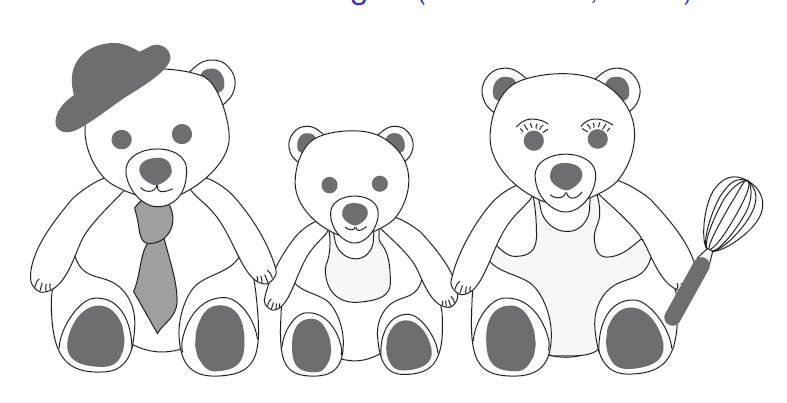
\includegraphics[scale=0.5]{img/struc_4.png}
\end{figure}

\subsubsection{Strukturvererbung}
\begin{framed}
	\textbf{Definition 6 - Strukturvererbung: Klassen- und Typhierarchie}
	\begin{description}
		\item $K_1$ Unterklasse von $K_2$, wenn Extension zu $K_1$ Teilmenge der Extension zu $K_2$
		\item $T_1$ Untertyp von $T_2$, wenn $T_1$ mehr Komponenten hat als $T_2$ (Definition vereinfacht für $T$ Tupeltyp)
	\end{description}
\end{framed}

\begin{itemize}
	\item nach DB-Entwurf: beide Hierarchien parallel
	\item nach Anfragen: Hierarchien müssen nicht mehr übereinstimmen
	
	\item \textbf{Einordnung:}
	\begin{itemize}
		\item OOPLs: $K_1$ Unterklasse von $K_2$m wenn $K_1$ die Methoden von $K_2$ erbt (nutzt die Impl. von $K_2$)
		\item etwa mgl: BAG Unterklasse von SET, da BAG Impl von SET nutzt, konzeptuell ist SET Unterklasse von BAG
	\end{itemize}
	
	\begin{figure}[!h]
		\centering
		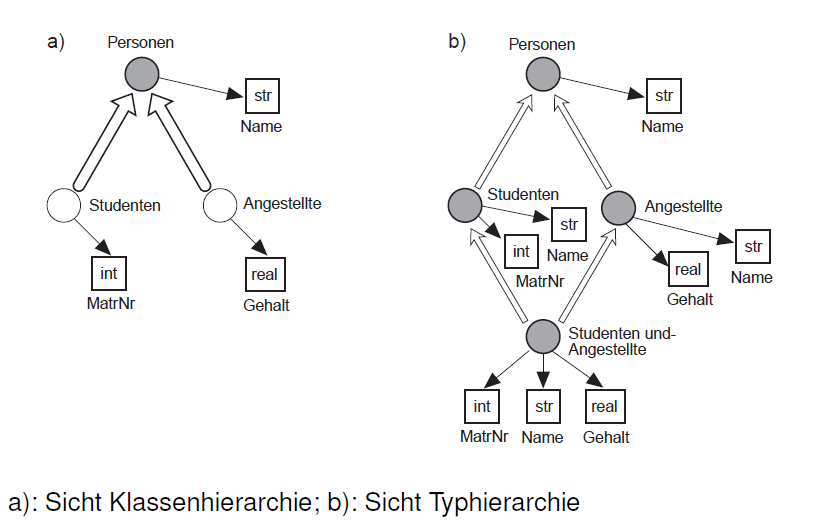
\includegraphics[scale=0.6]{img/struc_inheritance_ex.png}
	\end{figure}
	
	\item \textbf{OODB-Begriffe}
	\begin{table}[!h]
		\centering
		\begin{tabular}{|p{10em}|p{15em}|p{15em}|}
			\hline
			Begriffe	& Bedeutung in OOPLs	& Bedeutung in OODMs\\
			\hline
			\hline
			Klassenhierarchie	& Vererbung der Implementierung	& Integritätsbedingungen\\
			\hline
			Typhierarchie	& Gleiches Verhalten, mehr anwendbare Attribute	& Gleiches Verhalten, mehr anwendbare Attribute\\
			\hline
			IST-Hierarchie	& Integritätsbedingung	& Integritätsbedingung und gleiches Verhalten\\
			\hline
			Spezialisierung	& wie IST-Hierarchie	& Festlegung der Domäne von Oberklassen\\
			\hline
			Generalisierung	& invers zu Spezialisierung	& Festlegung der Domäne von Oberklassen\\
			\hline
			\hline
			allgemein	& ohne Wertvererbung	& mit Wertvererbung\\
			\hline
		\end{tabular}
	\end{table}
	
	\item \textbf{Spezialisierung und Generalisierung}\\
	in OODB: beides spezieller Arten der Klassenhierarchie
	\begin{itemize}
		\item Spezialisierung
		\begin{itemize}
			\item Oberklasse (abstrakt oder frei) gegeben
			\item Unterklassen sind Teilmengen (frei)
		\end{itemize}
		
		\item Generalisierung
		\begin{itemize}
			\item Unterklassen (abstrakt oder frei) gegeben
			\item Oberklasse ist Vereinigung (frei)
		\end{itemize}
		
		\item Beispiele
		\begin{itemize}
			\item Spezialisierung von Personen (abstrakt) zu Studenten (frei)
			\item Spezialisierung von Studenten (frei) zu Hilfsassistenten (frei)
			\item Generalisierung von Studenten und Angestellte (beide frei) zu Entleiher (frei)
			\item Generalisierung von Angestellte (frei) und Geräte (abstrakt) zu Haushaltspositionen (frei)
		\end{itemize}
	\end{itemize}
	
	\item \textbf{Problem: Mehrfachvererbung}\\
	Lösung wie in OOPLs
	
	\item \textbf{Flache und tiefe Extension}
	\begin{itemize}
		\item flach: alle Extensionen sind disjunkt (in OOPLs üblich)
		\item tief: simuliert Mehrfachzugehörigkeit von Objekten zu Klassen
		\item aber kein allgemeines Inklusionsprinzip (da disjunkter Durchschnitt)
		\item Objekte werden immer in speziellster Klasse erzeugt
	\end{itemize}
\end{itemize}

\begin{figure}[!h]
	\centering
	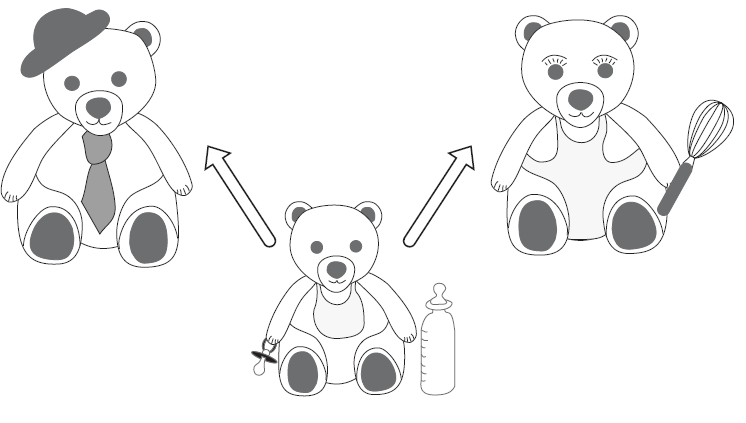
\includegraphics[scale=0.5]{img/struc_5.png}
\end{figure}

\subsubsection{Integritätsbedinungen}
\begin{framed}
	\textbf{Definition 7 - Integritätsbedingungen}
	\begin{description}
		\item \textbf{Schlüssel}
		\begin{itemize}
			\item vererbte Schlüssel (bei Personen definieren, bei Unterklassen nicht nötig)
			\item komplexe Schlüssel (Titel und Menge von Autoren bei Büchern)
			\item Schlüssel von Komponenten (Titel von Buch und Name von Verlag)
			\item andere Identifizierungsmechanismen (Klassenzugehörigkeit)
		\end{itemize}
		
		\item \textbf{Kardinalitäten}
		\begin{itemize}
			\item Nullwerte oder nicht
			\item Beziehungen 1:1, 1:n, m:n, meist asymmetrisch simuliert: Klassen und Komponentenklassen 
			\item Mengenkardinalitäten (student darf max 10 Bücher ausleihen, muss min drei VL hören); Vorsicht: unentscheidbar
		\end{itemize}
		
		\item Integritätsbedingungen an die Strukturvererbung
		\begin{itemize}
			\item Überdeckungsbedingung: außer Angestellten, Studenten gibt es keine weiteren Personen
			\item Disjunktheitsbedingung: Angestellte, Studenten sind disjunkt
		\end{itemize}
	\end{description}
\end{framed}

\begin{figure}[!h]
	\centering
	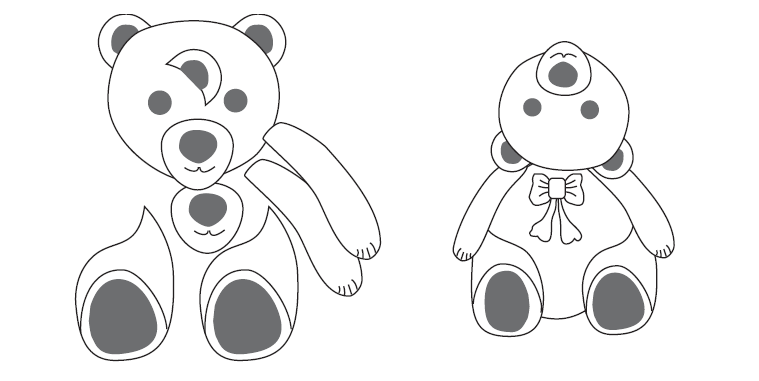
\includegraphics[scale=0.5]{img/struc_6.png}
	\caption{Auswirkung fehlender Integritätsbedingungen}
\end{figure}


\subsection{Operationenteil eines objektorientierten Datenbankmodells}
\begin{itemize}
	\item min die Möglichkeiten wie in SQL
	\item relationale Semantik: man extrahiert Werte aus Zuständen von Objekten\\
	Ergebnis ist geschachtelte Relation
	\item objekterzeugende Semantik:: man erzeugt neue Objekte als Anfrageergebnis mit Zuständen, die von vorhandenen Objekten extrahiert wurden\\
	Ergebnis ist eine dynamisch erzeugte Klasse
	\item objekterhaltende Semantik: man erhält eine Auswahl der in der DB vorkommenden Objekte mit neuen Zuständen\\
	Ergebnis ist dynamisch erzeugte Ober/Unterklasse
	
	\item \textbf{Einordnung, Unterschiede}
	\begin{itemize}
		\item Relationenmodell: generische Anfragen und Updates auf flachen Relationen
		\item OODBSs: Standard-Methoden auf COLLECTION-Klassen (Selektionen mit sehr einfachen Selektsionsprädikaten)\\
		OSQL mit relationaler Semantik (nicht so mächtig wie Std-SQL)
	\end{itemize}
	
	\item Taxonomie generischer Operationen
	\begin{figure}[!h]
		\centering
		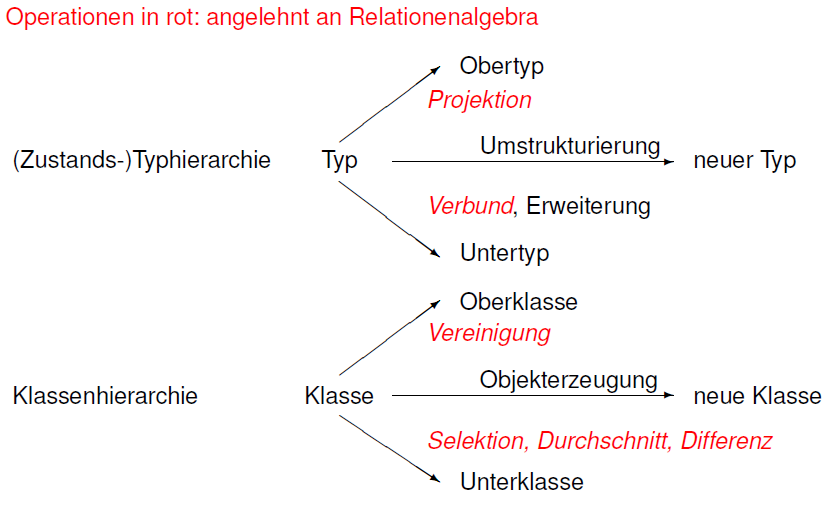
\includegraphics[scale=0.6]{img/taxonomie_generic_ops.png}
		\caption{Taxonomie generischer Operationen}
	\end{figure}
	
	\item Relationale Operationen
	\begin{itemize}
		\item Relationenalgebra
		\item Minimale geschachtelte Algebra (auf geschachtelten Relationen)
		\item orthogonal geschachtelte Algebra
		\item PNF-Algebra (auf geschachtelten Relationen in PNF = Partitioned Normal Form): bewahren Schlüssel, können also auch Objektidentitäten (und damit Objektrelationen) bewahren
	\end{itemize}
	
	\item \textbf{Anfragen:} klassenbasiert oder extensionsbasiert
	\begin{itemize}
		\item \textbf{Klassenbasierte Anfragen}
		\begin{itemize}
			\item bei objekterhaltender Semantik: man erhält eine Auswahl der in der DB vorkommenden Objekte mit neuen Zuständen
			\item Ergebnis ist dynamisch erzeugte Ober/Unterklasse
		\end{itemize}
		
		\item \textbf{Extensionsbasierte Anfragen}
		\begin{itemize}
			\item bei objekterhaltender Semantik: man erhält eine Auswahl der in der DB vorkommenden Objekte mit neuen Zuständen
			\item Ergebnis ist eine neue Extension einer bereits bestehenden Klassen
		\end{itemize}
		
		\item Beispiel:
		\begin{itemize}
			\item Selektion auf Klasse Studenten nach Studiengang 'Informatik'
			\item Klassenbasiert: Unterklasse Informatiker von Klasse Studenten
			\item Extensionsbasiert: Neue Extension Informatiker zur existierenden Klasse Studenten
		\end{itemize}
	\end{itemize}
\end{itemize}


\subsection{Höhere Konzepte eines objektorientierten Datenbankmodells}
\begin{itemize}
	\item höhere Konzepte: formal nur in Prädikatenlogik höherer Ordnung beschreibar (Struktur- und Operationenteil in 1. Ordnung)
	\item Methoden:\\
	Schnittstellen, Impl, Einkapselung, Vererbung, Overriding, Mehrfachvererbung, Konfliktauflösung
	\item Metaklassen
	
	\item \textbf{Methoden}
	\begin{itemize}
		\item Anfrage- und Update-Methoden\\
		Anfragen liefern neues (abgeleitetes Attribut) bel. Typs\\
		Updates liefern Fehlercode, Seiteneffekt: Änderung des Zustands des aktuellen Objekts
		
		\item Schnittstelle: Ein- und Ausgabeparameter, ihre Typen\\
		Impl: meist in OOPL (eingekapselt)
		
		\item Folgende Konzepte wie in OOPLs\\
		Vererbung, Overriding, Einkapselung, Mehrfachvererbung, Konfliktauflösung
	\end{itemize}
	
	\newpage
	\item \textbf{Varianten der Einkapselung}
	\begin{figure}[!h]
		\centering
		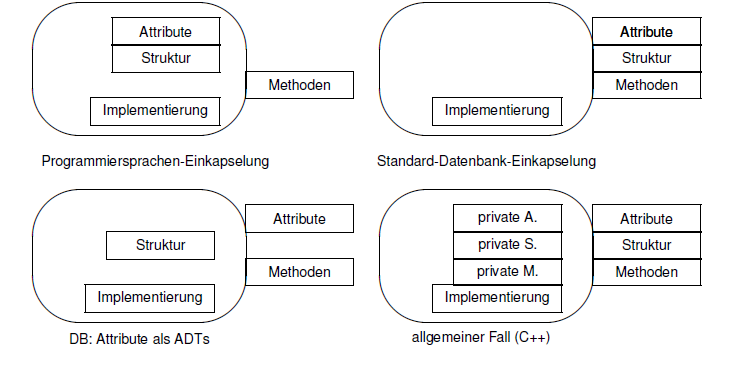
\includegraphics[scale=0.6]{img/einkapselung.png}
		\caption{Varianten der Einkapselung}
	\end{figure}
	
	\item \textbf{Overriding von Schnittstellen}\\
	bisher: Ersetzen von Impl.\\
	jetzt auch: kontrolliertes Ersetzen von Schnittstellen\\
	Notation: O - Methode der Oberklasse; U - Methode der Unterklasse
	
	\begin{figure}[!h]
		\centering
		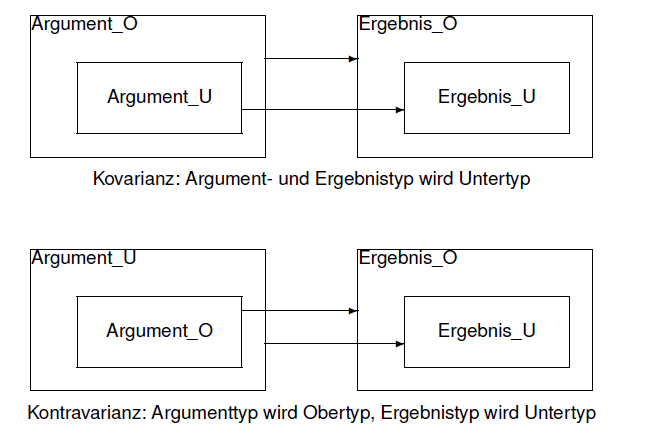
\includegraphics[scale=0.6]{img/ko_varianz.png}
	\end{figure}
	
	\item \textbf{Ko- und Kontravarianz}
	\begin{itemize}
		\item Kovarianz (Eiffel)\\
		Argument(typ) + Ergebnis(typ) wird jeweils Untertyp\\
		sinnvoll, aber nicht typsicher
		
		\item Kontravarianz\\
		Argument(typ) wird Obertyp, Ergebnis(typ) wird Untertyp\\
		nicht sinnvoll, aber typsicher
		
		\item No-Varianz (C++)\\
		Argument(typ) und Ergebnis(typ) bleiben unverändert
	\end{itemize}
	
	\item \textbf{Metaklassen}
	\begin{itemize}
		\item Klassen werde als Objekte (Instanzen) einer höheren Klasse (Metaklasse) aufgefasst
		\item dem Objekt (der Klasse) können dann Zustände zugewiesen werden, auf dem Objekt (af der Klasse) können Methoden ausgeführt werden
		\item in OOPLs:\\
		Klassenattribute statt Instanzattribute\\
		zb C++ statische Var mit static
		\item Anwendung: setzen Defaultwerte
		
		\item Anwendung: Methodendefinition\\
		höhere Konzepte = Beschreibbar in Prädikatenlogik > 1. Ordnung
	\end{itemize}
	
	\begin{figure}[!h]
		\centering
		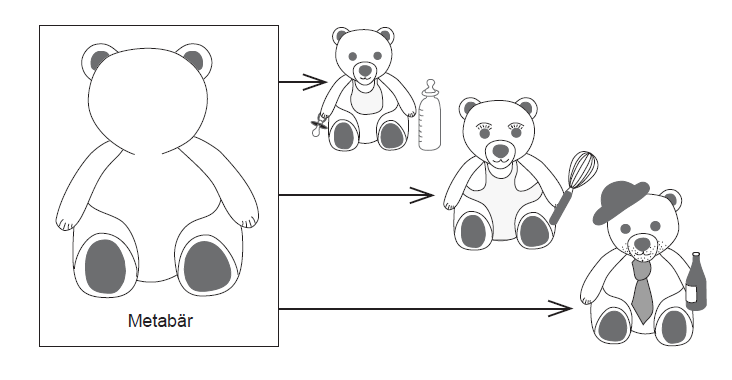
\includegraphics[scale=0.6]{img/metaclasses.png}
	\end{figure}
	
	\item \textbf{Instanzbeziehungen}
	\begin{itemize}
		\item neben Klasse-Unterklasse Beziehung (IST, INHERIT, Strukturvererbung, Klassenhierarchie) und
		\item Klasse-Komponentenklasse-Beziehung (IS\_PART\_OF) auch
		\item IS\_INSTANCE\_OF: Klasse-Instanz-Beziehung oder kurz Instanzbeziehung
	\end{itemize}
	
	\item \textbf{Einige formale Definitionen}
	\begin{framed}
		\textbf{Definition 8 - Typen, Typenkonstruktoren}
		\begin{description}
			\item Ein Typ ist ein Standard-Datentyp $T$, dem eine unstrukturierte Menge $dom(T)$ zugeordnet wird, oder ein konstruierter Typ:
			\begin{itemize}
				\item $T = \textrm{tuple of}(A_1: T_1, \ldots, A_n: T_n)$, wobei $T_1, \ldots, T_n$ wiederum Typen sind und $dom(T) = dom(T_1) \times dom(T_n)$ gilt,
				\item $T = \textrm{set of}(T_1)$ (oder auch $T = \textrm{set of} (A_1:T_1)$), wobei $T_1$ wiederum ein Typ ist und $dom(T) = \rho(dom(T_1))$ gilt,
				\item $T = \textrm{list of}(T_1)$ (oder auch $T = \textrm{list of} (A_1: T_1)$), wobei $T_1$ wiederum ein Typ ist und $dom(T) = T_1^*$ gilt.
			\end{itemize}
		\end{description}
	\end{framed}
	
	\begin{framed}
		\textbf{Definition 9 - abstrakte Domäne und Objektidentitäten}
		\begin{description}
			\item Sei $\mathbb{D}_\mathbb{A}$ eine Menge disjunkter, unendlicher Mengen $D_A$. Dann nennen wr jedes $D_A$ eine abstrakte Domäne. Jedes Element von $D_A$ ist eine Objektidentität (oder ein (abstraktes) Objekt).
		\end{description}
	\end{framed}
	
	\begin{framed}
		\textbf{Definition 10 - Zustandstyp und Zustand}
		\begin{description}
			\item Jedem (abstrakten) Objekt (oder jeder Objektidentität) wird ein komplexer Typ $T$ als Zustandstyp funktional zugeordnet. Der Zustand eines Objektes ist dann eine Instanz seines Zustandstyps.
		\end{description}
	\end{framed}
	
	\begin{framed}
		\textbf{Definition 11 - Klasse, Abstrakte Klasse, Extension}
		\begin{description}
			\item Ein gegebener Anwendungs-Objekttyp wird durch eine Klasse $K$ aus
			der Menge aller Klassen $\mathbb{K}$ repräsentiert. Jeder Klasse wird eine
			Domäne, eine Extension, ein Zustandstyp und eine Zustandsfunktion
			zugeordnet. Wird $K$ eine abstrakte Domäne als Domäne zugeordnet,
			so bezeichnen wir $K$ als abstrakte Klasse. Die Zuordnung geschieht
			über die Funktion dom mittels $dom : \mathbb{K} \to \mathbb{D_A}$. Die aktuelle Extension
			einer Klasse $o(K)$ ist eine Teilmenge von $dom(K)$. Wird $K$ keine
			abstrakte Domäne zugeordnet, so heißt $K$ freie Klasse.
		\end{description}
	\end{framed}
	
	\begin{framed}
		\textbf{Definition 12 - Zustandstyp einer Klasse, Zustandsfunktion}
		\begin{description}
			\item Jeder Klasse $K$ wird ein Zustandstyp $T_K$ funktional zugeordnet, der ein
			Standard-Datentyp, wiederum eine Klasse oder ein komplexer Typ ist.
			Ist im Zustandstyp eine Klasse enthalten, so wird diese Klasse
			Komponentenklasse von $K$ genannt. Jedem Objekt $\alpha$ aus der
			Extension $o(K)$ wird mittels der Zustandsfunktion ZUSTAND ein
			Element $w$ von $T_K$ zugeordnet. Dabei ist das Element von $T_K$ aus der
			Domäne des Typs bei Standard- und komplexen Typen und aus der
			Extension der Klasse bei Komponentenklassen. $w$ wird Zustand von $\alpha$ genannt.
		\end{description}
	\end{framed}
	
	\begin{framed}
		\textbf{Definition 13}
		\begin{description}
			\item Die Menge aller Klassen $\mathbb{K}$ sei partitioniert in die Menge aller abstrakten
			Klassen $\mathbb{K_A}$ und die Menge aller freien Klassen $\mathbb{K_F}$.
			Die Menge aller Spezialisierungen ist eine binäre Relation $spec$ über
			Klassen. Für jedes Element $K_1 spec K_2$ gilt, dass $K_1$ eine freie Klasse sein
			muss.\\
			Die Menge aller Generalisierungen ist eine binäre Relation $gen$ über Klassen.
			Für jedes Element $K_1 gen K_2$ gilt, dass $K_2$ eine freie Klasse sein muss.
			Die reflexive und transitive Hülle von $spec \cup gen$ wird mit $\leq$ bezeichnet und
			Klassenhierarchie genannt. Es wird zusätzlich gefordert, dass $\leq$ eine partielle
			Ordnung auf Klassen ist.
			Für jede freie Klasse $K$ definieren wir die Domäne durch
			\[dom(K) := \cap_{(K, K_i) \in spec} o(K_i) \textrm{ oder } dom(K) := \cup_{(K_i, K)\in gen} o(K_i)  \]
			wobei $o(K_i)$ die Extension der Klasse $K_i$ ist. Im zweiten Fall wird oft die Überdeckungsbedingung, also $o(K) = \cup_{(K_i, K)\in gen} o(K_i)$ gefordert.
		\end{description}
	\end{framed}
	
	Man beachte, dass in der letzten Definition jeder Klasse genau eine
	wohldefinierte Domäne zugeordnet wird, falls folgende
	Zusatzeinschränkungen getroffen werden (die in den Modellen IFO
	und EXTREM vorhanden sind):
	
	\begin{itemize}
		\item Jede freie Klasse taucht wenigstens einmal entweder auf der
		linken Seite eines $spec$-Tupels oder auf der rechten Seite eines
		$gen$-Tupels auf.
		\item Jeder Pfad aus $spec$-Tupeln, der in einer bestimmten Klasse $K$
		startet, endet in derselben Klasse $K'$.
		\item Die binäre Relation $spec \cup gen^{-1}$ ergibt einen gerichteten,
		azyklischen Graphen. Man beachte, dass zur Kontrolle der
		Azyklizität die Richtung der $gen$-Tupel umgedreht werden muss.
		Andreas
	\end{itemize}
	
	Die entsprechende Typhierarchie kann nun aus der Klassenhierarchie
	abgeleitet werden: alle in Oberklassen spezifizierten Attribute sind
	implizit auch für die Unterklassen definiert. Zunächst gehen wir davon
	aus, dass die jeweiligen Attributmengen disjunkt sind.
	
	\begin{framed}
		\textbf{Definition 14 - Vervollständigter Zustandstyp, Typhierarchie}
		\begin{description}
			\item Sei $K \leq K_1, K \leq K_2, \ldots K \leq K_p$ gegeben, dabei seien $K_1, K_2, \ldots, K_p$ alle direkten Oberklassen von $K$. 
			Dann ist der vervollständigte
			Zustandstyp von $K$ der Tupeltyp, der durch Konkatenation der
			vervollständigten Zustandstypen von $K_1, K_2, \ldots, K_p$ entsteht. Dann gilt:
			Ist $K \leq K'$, dann ist der vervollständigte Zustandstyp von $K$ Untertyp
			vom vervollständigten Zustandstyp von $K'$. Die Zustandstypen stehen
			dann bezüglich $\leq$ in einer Typhierarchie zueinander.
		\end{description}
	\end{framed}	
	
\end{itemize}


\subsection{Klassifikation objektorientierter Datenbanksysteme}
\begin{itemize}
	\item Entwicklungsrichtungen\\
	OO Datenbankprogrammiersprachen (OODBPLs)\\
	Objektrelationale Datenbanksysteme (ORDBMSs)\\
	Neuentwicklungen
	
	\item Andere Einteilung\\
	OO (OODGMSs): OODBPLs; Neuentwicklungen (native OODBMSs)\\
	Objektrelational (ORDBMSs): erweitert relational (nur Typkonstruktoren und Objektidentität); voll objrektrelational; offen, Wrapper oder Mapper
	
	\item Entwicklungen und Herausforderungen
	\begin{itemize}
		\item OOPLs $\to$ OODBSs: OOPL erweitern um\\
		Strukturteil: Extension, Persistenz, Typen,...\\
		Operationenteil\\
		Speicherungsstrukturen, Zugriffspfade, Transaktionen, Concurrency Control
		
		\item RDBSs $\to$ OODBSs: relationales DBS erweitern um\\
		Strukturteil (Typkonstruktoren, Objektidentität, Klassen, Klassen-/Typhierarchie)\\
		Methoden, Vererbung, Overriding
		
		\item Völlige Neuentwicklungen\\
		nicht OOPL oder relationales Datenmodell als Basis; eigenes OODM
	\end{itemize}
	
	\item \textbf{OODBPLs}
	\begin{itemize}
		\item Basis: C++, Smalltalk, CLOS, Java
		\item Standard: ODMG-Bindings
		\item Bsp: ObjectStore\\
		setzt Persistenzkonzept von Atkinson um (siehe Kap 5)\\
		Effizienz bei Zugriffen auf komplexe Objekte
		\item Nachteile: kein Operationenteil, kein Sichtkonzept\\
		nur Strukturteil (eingeschränkte Implementierungshierarchie) und Verhaltensteil verwirklicht\\
		dadurch starke Einschränkungen in Anwendungsmodellierung\\
		keinen Ebenentrennung: Speicherstrukturen, Sperren sichtbar
	\end{itemize}
	
	\item \textbf{ORDBMS}
	\begin{itemize}
		\item Basis: Relationenmodell
		\item Standard: SQL:1999,..., SQL:2011
		\item Objektrelationale DBS\\
		Relationen mit Klassen, Methoden, Klassen- und Typhierarchie\\
		Bsp: POSTGRES, alle großen RDBMS wie Oracle, DB2
	\end{itemize}
	
	\item Wann ist ein System objektrelational?\\
	umstrittene Quadrantenqualifikation nach Stonebreaker
	\begin{table}[!h]
		\centering
		\begin{tabular}{|l||l|l|}
			\hline
			& einfache Daten & komplexe Daten\\
			\hline
			\hline
			Anfragen	& relationale DB	& Objektrelationale DB\\
			\hline
			keine Anfragen	& Dateisysteme & Objektorientierte DB\\
			\hline
		\end{tabular}
	\end{table}
	besser: nach Standard SQL:1999 oder SLQ:2003
	\begin{figure}[!h]
		\centering
		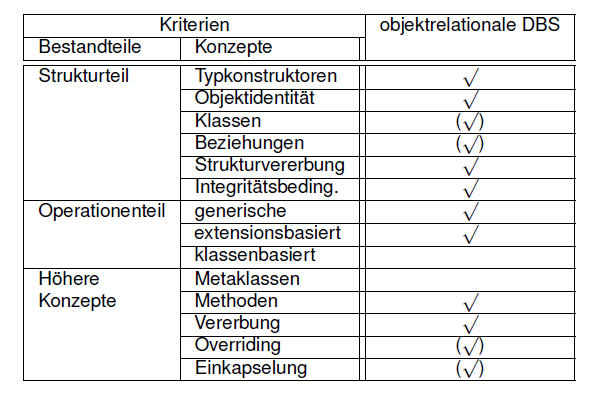
\includegraphics[scale=0.5]{img/objektrelational.png}
	\end{figure}
	
	\item \textbf{Objektrelationale Strukturen}
	\begin{itemize}
		\item relationales Datenmodell
		\item Drei-Ebenen-Architektur: volle Datenunabhängigkeit und Flexibilität mgl
		\item als Typen jedoch ADTs mit Typhierarchie, Methoden, evtl Overriding
		\item Objektidentitäten, Klassen oder Relationen (Tabellen)
		\item Klassen- oder Relationenhierarchien (Tabellenhierarchien)
		\item jedoch grundlegender Datentyp (auch für Anfragen): Relationen
	\end{itemize}
	
	drei Architekturen objektrelational
	\begin{itemize}
		\item OO-Schnittstelle auf RDBS: Wrapper (zb hibernate)
		\item RDBS mit internen ADT-Erweiterungen: halboffen (DB2, Oracle)
		\item RDBS mit externen ADT-Erweiterungen: offenes ORDBMS (Informix)
	\end{itemize}
	
	\begin{figure}[!h]
		\centering
		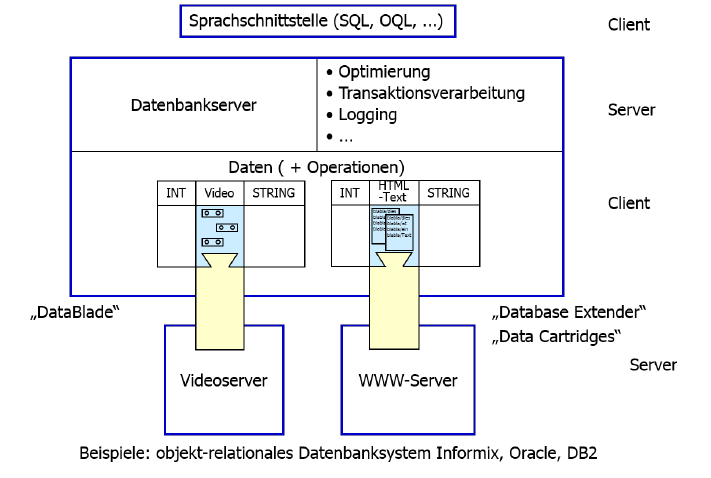
\includegraphics[scale=0.6]{img/open_ordbms.png}
	\end{figure}
	
	\item \textbf{Nachteile objektrelationaler Systeme}
	\begin{itemize}
		\item weiterhin Impedance Mismatch zu OOPL-Umgebungen
		\item oft Etikettenschwindel (nur DBS mit ADTs): noch große Unterschiede zw geplantem Standard SQL4, verabschiedetem Standard SQL:2003 und realen ORDBMS
		\item Anfragen/Sichtkonzept unterstützen relationale, aber nicht di eobjektorientierten Anteile im Modell
		\item Persistenzprinzip eingeschränkt: nur Tupel in Relationen persistent
	\end{itemize}
	
	\item \textbf{Neuentwicklungen}
	\begin{itemize}
		\item Basis: eigenes OODM\\
		nicht: Relationen mit Objekttypen und Objektidentität\\
		nicht OOPL-Klassen wie C++ und Smalltalk
		
		\item $O_2$\\
		zunächst OODM wie in VL\\
		danach Klassenhierarchie durch Typhierarchie ersetzt\\
		danach Verzicht auf Extensionen\\
		aber: Persistenz durch Namenskonzept, Erreichbarkeit
		
		\item \textbf{ITASCA}
		\item \textbf{OSCAR}
		
		\item keine dieser Entwicklung hat überlebt (Stand 2015)
	\end{itemize}
	
	\item Wie sieht es aktuell aus?\\
	Relationale DBSs $\to$ OODBSs? PostgreSQL, IBM DB2 ab V2, Oracle ab V8\\
	aktuelle Richtungen: NoSQL, Postrelationale DBS, Dokumentorientierte DBS
\end{itemize}